\chapter{Numerical Algorithms}\label{sec:numerics}

The system of equations is written as
\begin{equation}
  \frac{\partial \mathbf{q}}{\partial t} = \mathbf{f}_q(\mathbf{q},
  \boldsymbol{s},t) \;,\qquad
  \frac{\partial \mathbf{s}}{\partial t} = \mathbf{f}_s(\mathbf{q},
  \boldsymbol{s},t) \;,
\label{equ:problem}
\end{equation}
where $\boldsymbol{q}$ and $\boldsymbol{s}$ are the flow and scalar vectors. For the compressible formulation, we have
\begin{equation}
  \mathbf{q} = (\rho, \rho u_1, \rho u_2, \rho u_3, \rho e)^T \;,\qquad
  \mathbf{s} = (\rho s_1, \rho s_2, \ldots)^T \;.
\end{equation}
The energy equation can be also solved in terms of the total energy per unit volume $\rho(e+v^2/2)$ instead of the internal energy per unit volume $\rho e$. For the incompressible equations, we have
\begin{equation}
  \mathbf{q} = (u_1, u_2, u_3)^T \;,\qquad
  \mathbf{s} = ( s_1, s_2, \ldots)^T \;.
\end{equation}

The basic formulation is the method of lines, so that the algorithm is a combination of different spatial operators that calculate the right-hand side of the equations (typically, derivatives) and a time marching scheme. An implicit treatment of the diffusive terms in the incompressible case has also been implemented.

%%%%%%%%%%%%%%%%%%%%%%%%%%%%%%%%%%%%%%%%%%%%%%%%%%%%%%%%%%%%%%%%%%%%%%%%%%%%%%%%
%%%%%%%%%%%%%%%%%%%%%%%%%%%%%%%%%%%%%%%%%%%%%%%%%%%%%%%%%%%%%%%%%%%%%%%%%%%%%%%%
\section{Spatial operators}

Spatial operators are based on finite difference methods (FDM). There are two levels of routines. The low-level libraries contain the basic algorithms and are explained in this section. It consists of the FDM kernel library {\tt fdm} and three-dimensional operators library {\tt operators}. The high-level library {\tt fields} is composed of routines that are just a combination of the low-level routines.

\subsection{Derivatives}\label{sec:fdm}

See file {\tt operators/opr\_partial}. Spatial derivatives are calculated using fourth- or sixth-order compact Pad\'{e} schemes as described by \cite{Lele:1992} and \cite{Lamballais:2011} for uniform grids and extended by \cite{Shukla:2005} for non-uniform grids. The kernels of the specific algorithms are in the library {\tt fdm}.

We consider FD approximations
\begin{equation}
  a_{-1}s'_{j-1}+a_{0}s'_{j}+a_{+1}s'_{j+1}=\sum_{k=-2}^{k=2}b_ks_{j+k} \;,\qquad
  a_{-1}s''_{j-1}+a_{0}s''_{j}+a_{+1}s''_{j+1}=\sum_{k=-3}^{k=3}b_ks_{j+k} \;.
  \label{equ:coefs}
\end{equation}
$\{s_j:\, j=1,\ldots,n\}$ are the values of the function $s(x)$ evaluated at $x_j\in[x_1\,,x_n]$. The sets $\{s'_j\}$ and $\{s''_j\}$ denote approximations to the first- and second-order derivatives evaluated at $\{x_j\}$. For the first-order derivatives, we have a 5-point stencil. For the second-order derivatives, we have a 7-point stencil. The coefficients for the first-order derivative are given in table~\ref{tab:coeffs1}. The coefficients for the first-order derivative are given in table~\ref{tab:coeffs2}.

\begin{table}[!ht]
  \small
  \centering
  \begin{tabular}{l@{\hspace{6ex}}ccc@{\hspace{6ex}}ccccc@{\hspace{6ex}}c}\hline
    &$a_{-1}$&$a_{0}$&$a_{+1}$&$b_{-2}$&$b_{-1}$&$b_{0}$&$b_{+1}$&$b_{+2}$&$t$\\ \hline
    C2&0        &1&0       & 0 & $^{-1}\!/\!_2$ & 0 &$^1\!/\!_2$ & 0&
    $\;\,^{1}\!/\!_{3!}\,h^2s^{(3)}$\\
    C4&$^1\!/\!_4$&1&$^1\!/\!_4$& 0 &$ ^{-3}\!/\!_4$ & 0 &$^3\!/\!_4$ & 0&
    $^{-1}\!/\!_{5!}\,h^4s^{(5)}$\\
    C6&$^1\!/\!_3$&1&$^1\!/\!_3$&$ ^{-1}\!/\!_{36}$ &$ ^{-7}\!/\!_9$  & 0 &
    $^7\!/\!_9$  &$^{1}\!/\!_{36}$&
    $\;\,^{4}\!/\!_{7!}\,h^6s^{(7)}$\\
    B1&0      &1&0       & 0 & 0 & -1 & 1 & 0&
    $\;\,^{1}\!/\!_{2!}\,h\;\,s^{(2)}$\\
    B3&0      &1&2       & 0 & 0 & $^{-5}\!/\!_2$ & 2 &$ ^1\!/\!_2$&
    $^{-2}\!/\!_{4!}\,h^3s^{(4)}$\\
    B5&$^1\!/\!_6$&1&$^1\!/\!_2$& 0 &$ ^{-10}\!/\!_{18}$ &$ ^{-1}\!/\!_2$ & 1&
    $^{1}\!/\!_{18}$&$^{-2}\!/\!_{6!}\,h^5s^{(6)}$\\\hline
  \end{tabular}
  \caption{Coefficients of the finite-difference formulae (\ref{equ:coefs}) for the first-order derivative. The first three rows are centered differences, the last three are biased differences. The matrix $A_1$ in (\ref{equ:fdm}) is constructed in terms of the coefficients $\{a_i\}$, the matrix $B_1$ in terms of $\{b_i\}$. The last column contains the leading order term of the local truncation error defined by (\ref{equ:truncation1}).}
  \label{tab:coeffs1}
\end{table}

\begin{table}[!ht]
  \small
  \centering
  \begin{tabular}{l@{\hspace{6ex}}ccc@{\hspace{6ex}}ccccccc@{\hspace{6ex}}r}\hline
    &$a_{-1}$&$a_{0}$&$a_{+1}$&$b_{-3}$&$b_{-2}$&$b_{-1}$&$b_{0}$&$b_{+1}$&$b_{+2}$&$b_{+3}$&\multicolumn{1}{c}{$t$}\\
    \hline
    C2& 0&              1&  0&              0& 0& 1& -2& 1& 0& 0&
    $^{2}\!/\!_{4!}\,h^2s^{(4)}$\\
    C4& $^1\!/\!_{10}$& 1&  $^1\!/\!_{10}$& 0& 0& $^{6}\!/\!_5$& $^{-12}\!/\!_5$& $^6\!/\!_5$& 0& 0&
    $^{3}\!/\!_{5}\,^{1}\!/\!_{5!}\,h^4s^{(6)}$\\
    C6& $^2\!/\!_{11}$& 1&  $^2\!/\!_{11}$& 0& $^{3}\!/\!_{44}$& $^{12}\!/\!_{11}$& $^{-51}\!/\!_{22}$&
    $^{12}\!/\!_{11}$  &$^{3}\!/\!_{44}$& 0 &
    $^{-23}\!/\!_{11}\,^{1}\!/\!_{7!}\,h^6s^{(8)}$\\
    C6b& -& 1& -& -& -& -& -& -& -& -& -\\
    B1 &0      &1&0       & 0 & 0 & 0 & 1 & -2& 1 & 0 &
    $h\,s^{(3)}$\\
    B3 &0      &1&11       & 0 & 0 & 0& 13 & -27& 15 & -1 &
    $^{-2}\!/\!_{4!}\,h^3s^{(5)}$\\
    B5 &$^1\!/\!_{10}$&1&$^{-7}\!/\!_{20}$& 0& 0& $^{99}\!/\!_{80}$ & $-3$ & $^{186}\!/\!_{80}$& $^{-3}\!/\!_{5}$& $^{3}\!/\!_{80}$&
    $^{3}\!/\!_{5}\,^{1}\!/\!_{5!}\,h^5s^{(7)}$\\\hline
  \end{tabular}
  \caption{Coefficients of the finite-difference formulae (\ref{equ:coefs}) for the second-order derivative. The first three rows are centered differences, the last three are biased differences. The matrix $A_2$ in (\ref{equ:fdm}) is constructed in terms of the coefficients $\{a_i\}$, the matrix $B_2$ in terms of $\{b_i\}$. The last column contains the leading order term of the local truncation error defined by (\ref{equ:truncation1}).}
  \label{tab:coeffs2}
\end{table}

Global schemes are constructed as a combination of $n$ of these formulae, using biased finite differences at the boundaries in case of non-periodicity. For the first-order derivative, we define the global algorithm (35653) by using the centered scheme C6 at the $(n-4)$ interior points, and the biased schemes B5 at $j=2$ and B3 at $j=1$ with the corresponding symmetric counterpart at $j=n-1$ and $j=n$, respectively \citep{Carpenter:1993}. For the second-order derivative, we define the global algorithm (3466b43) by using the centered scheme C6b at the $(n-6)$ interior points, C6 at $j=3$ and $j=n-2$, C4 at $j=2$ and $j=n-1$, and the biased scheme B3 at $j=1$ with the corresponding symmetric counterpart at $j=n$. We tried the biased scheme B5 instead of the centered scheme C4 for $j=2$ and $j=n-1$; the eigenvalues were closer to the spectral case, but the truncation errors $e_j$ were larger despite $t_j$ begin smaller (see below).

We define the $n$-dimensional vectors
\begin{equation}
  \mathbf{s}^T=[s_1\;,\ldots s_n]\;,\qquad (\mathbf{s'})^T=(\delta_x \mathbf{s})^T=[s'_1\,\ldots s'_n]\;,\qquad (\mathbf{s''})^T=(\delta_{xx} \mathbf{s})^T=[s''_1\,\ldots s''_n] \;.
\end{equation}
The global schemes can be represented as
\begin{equation}
  A_1\, \delta_x \mathbf{s}=(1/h)B_1\, \mathbf{s} \;, \qquad
  A_2\, \delta_{xx} \mathbf{s}=(1/h^2)B_2\, \mathbf{s}
\label{equ:fdm}
\end{equation}
where $h=(x_n-x_1)/(n-1)$ is a reference space step and the square matrices $A=(a_{ij})$ and $B=(b_{ij})$ are narrow banded. If periodic boundary conditions are used, these are imposed at $x_{n+1}$ and not at $x_n$, i.e.  $s(x_{n+1})=s(x_1)$. The size of the domain is then $L=n(x_n-x_1)/(n-1)=nh$ instead of $x_n-x_1=(n-1)h$, and we do not save the information at $x_{n+1}$. The matrices $A$ and $B$ are then circulant instead of banded. The Thomas' algorithm is used to solve those linear systems. An LU decomposition is performed during the initialization and equations are normalized such that the right-hand side contains at least one diagonal of just ones, so as to save memory and computational time (see routine {\tt   fdm\_initialize}). For analysis, one can consider equation~(\ref{equ:fdm}) as the definition of linear finite-difference operators $\delta_x: \mathbb{R}^n \rightarrow \mathbb{R}^n$, $\mathbf{s'} = \delta_x\mathbf{s} = (1/h)(A_1^{-1}B_1)\mathbf{s}$, and $\delta_{xx}: \mathbb{R}^n \rightarrow \mathbb{R}^n$, $\mathbf{s''} = \delta_{xx}\mathbf{s} = (1/h^2)(A_2^{-1}B_2)\mathbf{s}$ \citep{Mellado:2012}.

The local truncation errors of the FD approximations~(\ref{equ:fdm}) to the first-order derivative, $\{e_{1,j}=ds/dx(x_j)-s'_j\,:\;j=1,\ldots,n\}$, are given by
\begin{equation}
  \mathbf{e_1} = -A_1^{-1}\mathbf{t_1}\;,\qquad
  \mathbf{t_1}=
  \frac{1}{h}B_1\left(\begin{array}{c}s(x_1)\\\vdots\\s(x_n)\end{array}\right)-
  A_1\left(
  \begin{array}{c}\frac{ds}{dx}(x_1)\\\vdots\\\frac{ds}{dx}(x_n)
  \end{array}\right)\;.
  \label{equ:truncation1}
\end{equation}
A similar expression can be derived for the second-order derivatives. The components of $\mathbf{t_1}$ and $\mathbf{t_2}$ can be found in table~\ref{tab:coeffs1} and table~\ref{tab:coeffs2}.

For notational convenience in the following discussion on Fourier analysis, we change the index so that it varies between $j=0$ and $j=n-1$. We can define a new sequence of numbers $\{\hat{s}_k\}_0^{n-1}$ from $\{s_j\}_0^{n-1}$ by
\begin{equation}
\hat{s}_k=\frac{1}{n}\sum_0^{n-1}s_j\exp(-i\omega_kj)\;,\qquad
s_j=\sum_0^{n-1}\hat{s}_k\exp(i\omega_kj)\;,
\label{equ:dft}
\end{equation}
where $\{\omega_k=(2\pi/n)k:\, k = 0,\ldots,n-1\}$ is the scaled wavenumber and $i=\sqrt{-1}$ is the imaginary unit. We use the library FFTW in the code for this transformation~\footnote{visit {http://www.fftw.org/}}. Note that $\hat{s}_{k+n}=\hat{s}_k$ because $\exp(-i2\pi j)=1$ for any integer number $j$, so that we can write
\begin{equation}
  s_j =  \sum_{-n/2+1}^{n/2} \hat{s}_k \exp[i\omega_kj]\;.
\end{equation}
The expression above coincides with the Fourier series $\sum_{-n/2}^{n/2} \hat{s}_k \exp[i\kappa_kx]$ of the function $s(x)$ over the interval $[0,L]$ particularized at the grid points $\{x_n\}$ provided that the spectral content of the function $s(x)$ beyond the Nyquist frequency $\kappa_{n/2}=(2\pi/L)(n/2)=2\pi/(2h)=\pi/h$ is zero. Then we have the relation $\kappa_kh=\omega_k$ between the wavenumber $\kappa_k=(2\pi/L)k$ and the scaled wavenumber $\omega_k$. In principle, both $\{\hat{s}_k\}$ from $\{s_j\}$ are complex numbers; however, the sequence $\{\hat{s}_k\}$ is typically real and we only need to know the Fourier modes between $k=0$, the mean value, and $k=n/2$, the Nyquist frequency, because of the symmetry. Then, $\omega_k$ varies between 0 and $\pi$ and $\kappa_k$ varies between 0 and $\pi/h$. A third quantity sometimes used in the discussion is the number of points per wavelength $\mathrm{PPW}_k=(L/k)/h=2\pi/\omega_k$; for a given wavelength $L/k$, or wavenumber $\kappa_k$, reducing the grid step $h$ and thus increasing resolution -- increasing $\mathrm{PPW}_k$ -- means reducing the scaled wavenumber $\omega_k$ towards zero.

With previous framework we can use von Neumann analysis to understand the properties of the FDM. We know that the exact values of $\{s'_j\}$ and $\{s''_j\}$ under the conditions stated above are
\begin{equation}
  s'(x_j) =\sum_0^{n-1} (i\omega_k/h)  \hat{s}_k\exp(i\omega_kj)\;,\qquad
  s''(x_j)=\sum_0^{n-1} (-\omega^2_k/h^2)\hat{s}_k\exp(i\omega_kj)\;,
\end{equation}
having used $\kappa_k=\omega_k/h$. The FDM approximations can be written as
\begin{equation}
  s'_j =\sum_0^{n-1} (\lambda_1/h)  \hat{s}_k\exp(i\omega_kj)\;,\qquad
  s''_j=\sum_0^{n-1} (\lambda_2/h^2)\hat{s}_k\exp(i\omega_kj)\;.
  \label{equ:lambda}
\end{equation}
The deviation of the complex functions $\lambda_1(\omega)$ and $\lambda_2(\omega)$ from the exact values $i\omega$ and $-\omega^2$ measures the FDM discretization error (see figure~\ref{fig:fdm}).  One possible way to quantify this error is by means of the resolving efficiency, defined as the number of points per wavelength PPW required to maintain errors in the corresponding transfer function below a specified level (or, equivalently, a specified error in the dispersion velocity of the linear advection problem). In these terms, for the first-order derivative, an error of 1\% requires 4 PPW in the case of the implicit compact scheme C6, whereas the second-order explicit scheme C2 requires 25 PPW \citep{Lele:1992,Lomax:1998}. This difference is even higher if the common reference error of 0.1\% is retained, for which the previous finite difference schemes require 6 PPW and 100 PPW, respectively. The corresponding resolution requirements for the second-order derivative using a compact scheme are similar to those of the first-order derivative; the second-order central explicit FDM improves slightly and only needs 18 PPW for 1\% error and 67 PPW for 0.1\% error. These errors in the transfer function can be understood as errors in the exponential rate of decrease of a given wave caused by the diffusion operator. The scheme compact b corresponds to the 7-point stencil described in \cite{Lamballais:2011}.
%However, these are theoretical values based on linear analysis of the algorithm and resolution studies are always required to ascertain this error.
Last, we also note that, as we increase resolution, $h$ decreases and $\omega_k$ moves towards the origin in figure~\ref{fig:fdm} for a fixed wavenumber $\kappa_k$; the departure at the origin of the approximation from the exact value gives then the order of the FDM.

\begin{figure}
  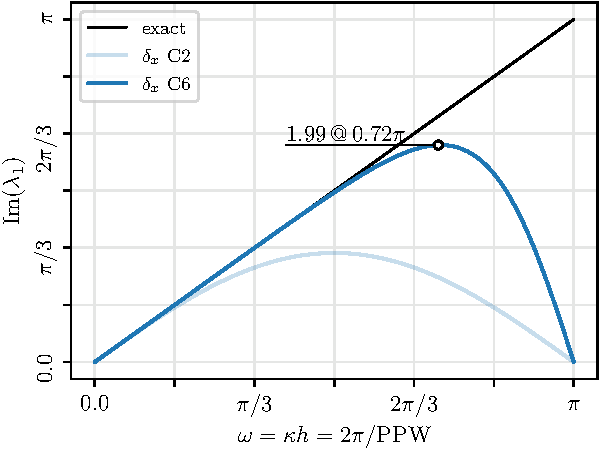
\includegraphics[clip,width=0.49\textwidth]{figs/fdm1}\hfill
  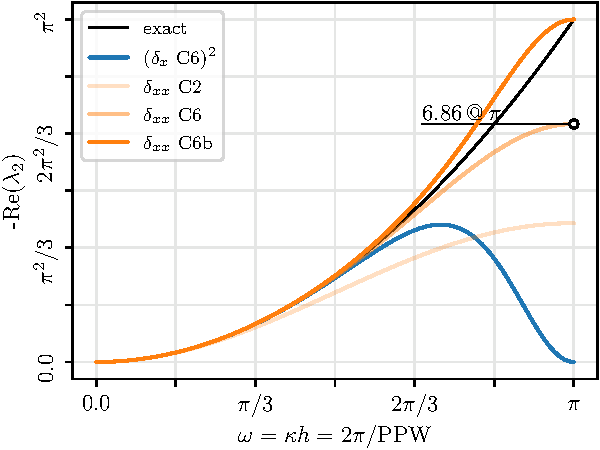
\includegraphics[clip,width=0.49\textwidth]{figs/fdm2}
  \caption{Modified wavenumbers of the FDM approximations to the (left) first-order derivative and (right) second-order derivatives. The blue line in right panel corresponds to the operator $\delta_{x}\delta_{x} =(A_1^{-1}B_1)^2$. The interval $[-\pi,0$ is simply the anti-symmetric extension in the left panel, and the symmetric extension in the right panel. The scheme compact a corresponds to the 5-point stencil in \cite{Lele:1992} and compact b corresponds to the 7-point stencil in \cite{Lamballais:2011}. The latter is the default scheme in the code.}
  \label{fig:fdm}
\end{figure}

It is also useful to use the notation
\begin{equation}
  \hat{\mathbf{s}} = W\, \mathbf{s}\,\qquad \mathbf{s}=W^{-1}\hat{\mathbf{s}}\;.
\end{equation}
for the discrete Fourier transform (DFT) defined by equation~(\ref{equ:dft}),
where $W$ is the DFT matrix. Let us consider the first-order derivative in
equation~(\ref{equ:fdm}). Then, we can write
\begin{equation}
  \hat{\mathbf{s'}}=W\, \mathbf{s'} =
  [(1/h)W(A_1^{-1}B_1)W^{-1})W\mathbf{s} = (1/h)\Lambda_1\hat{\mathbf{s}} \;.
\end{equation}
From this relation between the vectors $\hat{\mathbf{s'}}$ and $\hat{\mathbf{s}}$ and equation~(\ref{equ:lambda}), we deduce that the array $\Lambda_1$ is diagonal with $\{\lambda_k\}_0^{n-1}$ as diagonal elements. Moreover, since $W$ is invertible, $W$ represents just a similarity transformation -- a change of base -- and therefore we know that the matrices $A_1^{-1}B_1$ and $\Lambda_1$ have the same eigenvalues. Hence, $\{\lambda_k\}_0^{n-1}$ is simply the set of eigenvalues of $A_1^{-1}B_1$; figure~\ref{fig:fdm} shows the curve through the imaginary part of half of them. In the complex plane, the numbers $\{\lambda_{1,k}\}_0^{n-1}$ corresponding to the first-order derivative move in the imaginary axis, and the numbers $\{\lambda_{2,k}\}_0^{n-1}$ corresponding to the second-order derivative move in the negative part of the real axis.
%This exercise might not be relevant for the periodic case because we can obtain $\{\lambda_k\}_0^{n-1}$ easily by substituting equation~(\ref{equ:dft}) into equation~(\ref{equ:coefs}), but it is clarifying for the non-periodic cases because the equivalent of figure~\ref{fig:fdm} is simply the spectrum of $A_1^{-1}B_1$, in general, a set of points in the complex plane.

We can calculate the FD approximation to the second-order derivative as $\delta_{x}\delta_{x} \mathbf{s} = (A_1^{-1}B_1)^2$, that is, to consecutively apply the FD approximation to the first-order derivative twice. However, the spectral transfer function of the FD operator $\delta_{x}\delta_{x}$ falls to zero at the Nyquist frequency, as shown in figure~\ref{fig:fdm}, which results in a very poor representation of the diffusion terms at the high wavenumbers. This property can become very important because the errors derived from the aliasing in calculating the non-linear terms accumulate and the use of filter might become unavoidable to have stable simulations. Hence, we use a direct discretization of the second-order derivative operator, compact a or compact b.

Last, a uniform grid $\{x_j=x_1+(j-1)h:\, j = 1,\ldots,n\}$ has been considered so far. If a non-uniform grid $\{x_j:\, j = 1,\ldots,n\}$ is employed instead, we can define $\mathbf{x'} = (1/h)A_1^{-1}B_1\mathbf{x}$ from the mapping between the computational and the physical domains and the calculation of the approximation $\delta_{x} \mathbf{s}$ to the first-order derivative is given by
\begin{equation}\label{equ:nonuniform1}
  (A_1D_1)\, \delta_x \mathbf{s}=(1/h)B_1 \mathbf{s} \;,
\end{equation}
that is, $A_1$ should be replaced by $A_1D_1$, where $D_1=\text{diag} (\mathbf{x'})$ is a diagonal matrix with $\{x'_j\}$ as diagonal elements. Similarly, for the FD approximation to the second-order derivative, we obtain
\begin{equation}
  (A_2D_1^2)\, \delta_{xx} \mathbf{s}=(1/h^2)B_2 \mathbf{s} - (A_2D_2)\,\delta_x
  \mathbf{s} \;,
\end{equation}
where $D_2=\text{diag} (\mathbf{x''})$ is again a diagonal matrix with
$\{x''_j\}$ as diagonal elements; these elements are the components of the vector $\mathbf{x''} = (1/h^2)A_2^{-1}B_2\mathbf{x}$. As a result of using this Jacobian formulation for non-uniform grids, we need to calculate the approximation to the first-order derivative in order to calculate $\delta_{xx} \mathbf{s}$. In general, that is not a problem because we need both, the first- and the second-order derivatives, in all the transport equations.

We could reformulate the calculation of the second-order derivative as
\begin{subequations}\label{equ:nonuniform2}
  \begin{align}
    (A_2D_1^2)\, \mathbf{s}^*&=(1/h^2)B_2 \mathbf{s} \;,\\
    \delta_{xx} \mathbf{s}&= \mathbf{s}^*- (D_1^{-2}D_2)\,\delta_x  \mathbf{s} \;,
  \end{align}
\end{subequations}
where $D_1^{-2}D_2$ is a diagonal matrix and could be precomputed. This formulation is clearer and useful for the stability analysis, but not faster.

A direct formulation of compact FD approximation to the second-order derivative for non-uniform grids is needed, however, when using the implicit temporal scheme for the diffusion terms in order to solve exactly the corresponding Helmholtz equations, without any approximation. Such a direct formulation leads to the system form~(\ref{equ:fdm}). We followed \cite{Shukla:2005}.

\subsection{Advection and Diffusion}

The non-linear advection terms can be formulated in conservative, convective and skew-symmetric forms \citep{Blaisdell:1996,Kravchenko:1997}. The molecular transport terms can be formulated in the conservative and non-conservative forms (this latter if transport coefficients are constant).

In the convective formulation, the routines {\tt OPR\_BURGERS\_*} combine the first and second-order derivative operators as
\begin{equation}
f=\epsilon s'' - u s'\;
\end{equation}
where $s$ is a scalar field, $u$ a velocity field, and $\epsilon$ is the diffusivity. The combination reduces transpositions, either locally or across processors. The reason is that, in general, we need 2 transpositions for $s''$, forward and backward, and similarly for $s'$, which amounts to 4 transpositions. In the the combined form, we need 1 forward transposition for $s$ and 1 for $u$, and then 1 backward transposition for the result $f$. In total, 3 transpositions. The addition and multiplication operations are done in transposed space. If $u= s$, then it is only 2 transpositions that we need. When $u\ne s$, then the transposed velocity needs to be passed through the arguments in case it is needed.

In the anelastic mode, the operator calculates
\begin{equation}
f=\rho_\mathrm{bg}^{-1}\epsilon s'' - u s'\;,
\end{equation}
where $\rho_\mathrm{bg}$ is the background density profile.

We could reformulate the calculation of $\mathbf{f}$ by combining the linear operation with the calculation of the second derivative, which yields
\begin{equation}
    \epsilon^{-1}(A_2D_1^2)\, \mathbf{f}=(1/h)B_2 \mathbf{s}
    - A_2(D_2 + \epsilon^{-1}D_1^2\mathbf{u})\,\delta_x  \mathbf{s} \;,
\end{equation}
or
\begin{subequations}
  \begin{align}
    \epsilon^{-1}(A_2D_1^2)\, \mathbf{f}^*&=(1/h)B_2 \mathbf{s} \;,\\
    \mathbf{f}&= \mathbf{f}^*- (\epsilon D_1^{-2}D_2 + \mathbf{u})\,\delta_x  \mathbf{s} \;,
  \end{align}
\end{subequations}
where $\epsilon D_1^{-2}D_2$ is a diagonal matrix and could be precomputed. This formulation is clearer, but not sure if faster, and we need more memory because $\epsilon D_1^{-2}D_2$ varies with $\epsilon$.

\subsection{Filters}\label{sec:filters}

See file {\tt operators/opr\_filter}. The kernels of the specific algorithms are in the library {\tt filters}. Used in previous versions for long-term stability, filters are now mainly used for post-processing.

There are global filters and directional filters. Global filters are spectral filters in the horizontal plane, and Helmholtz-based filters. Band spectral filters remove the energy content outside a band $[\alpha_1,\alpha_2]$ in frequency space. Erf spectral filters are low- and high-pass filters defined at $\alpha_1$ with a thickness $\alpha_2$ in the logarithm of the frequency ($\alpha_1>0$ for high-pass filter, and $\alpha_1<0$ for low-pass filter). Helmholtz-based filters are defined by
\begin{equation}
  (1-\alpha^2\nabla^2) f = s \;,
\end{equation}
where $s$ is the original field, $f$ is the filtered field, and $\alpha=\lambda/(2\pi)$ where $\lambda$ is the filter size. This equation is transformed into the Helmholtz equation and solved as explained in section~\ref{sec:helmholtz}. This filter is motivated by the Navier-Stokes-alpha model \citep{Foias:2001}. Along the vertical non-periodic direction, we can impose Dirichlet or Neumann boundary conditions, where the former option maintains the value of the field at the boundary and the latter option imposes a zero gradient.

Directional filters are a sequence of one-dimensional filters in each direction. There are compact filters, which are implemented following \cite{Lele:1992}, and top-hat filters (or box filter), which are implemented using the trapezoidal rule to discretize the integral.

As an example of top-hat filter, let us consider a top-hat filter of a function $s(x)$ where the filter size is four times the grid size. Then, the value at the grid node $x_i$ of the filtered function $f(x)$ is
\begin{equation}
  f_i = \frac{1}{\Delta_{f,i}}\left\{\frac{s_{i-2}+s_{i-1}}{2}\Delta_{i-2}+
  \frac{s_{i-1}+s_{i}}{2}\Delta_{i-1}+\frac{s_{i}+s_{i+1}}{2}\Delta_{i}+
  \frac{s_{i+1}+s_{i+2}}{2}\Delta_{i+1}\right\}
\end{equation}
where
\begin{subequations}
  \begin{align}
    \Delta_i&=x_{i+1}-x_{i} \;,\\
    \Delta_{f,i}&=x_{i+2}-x_{i-2}=\Delta_{i-2}+\Delta_{i-1}+\Delta_{i}+\Delta_{i+1} \;.
  \end{align}
\end{subequations}
The linear operation can be written as
\begin{equation}
  f_i = c_{1,i}s_{i-2}+c_{2,i}s_{i-1}+c_{3,i}s_{i}+c_{4,i}s_{i+1}+c_{5,i}s_{i+2} \;,
\end{equation}
where the coefficients are
\begin{subequations}
  \begin{align}
    c_{1,i} &= (2\Delta_{f,i})^{-1} \Delta_{i-2}\;,\\
    c_{2,i} &= (2\Delta_{f,i})^{-1}(\Delta_{i-1}+\Delta_{i-2})\;,\\
    c_{3,i} &= (2\Delta_{f,i})^{-1}(\Delta_{i}+\Delta_{i-1})\;,\\
    c_{4,i} &= (2\Delta_{f,i})^{-1}(\Delta_{i+1}+\Delta_{i})\;,\\
    c_{5,i} &= (2\Delta_{f,i})^{-1}\Delta_{i+1}\;.
    \end{align}
\end{subequations}
For the tophat filter, we can imposed free or solid boundary conditions along the non-periodic directions. The former option uses ghost cells where the function is the linear extrapolation of $s(x)$ based on the values at the two nodes next to the boundary. The latter option uses ghost cells where the function is constant and equal to the boundary value of $s(x)$. As an example, consider the solid boundary near $i=1$ for the example above:
\begin{subequations}
  \begin{align}
    f_1 &= \tilde{c}_{3,1}s_{1}+c_{4,1}s_{2}+c_{5,1}s_{3} \;,\\
    f_2 &= \tilde{c}_{2,2}s_{1}+c_{3,2}s_{2}+c_{4,2}s_{3}+c_{5,2}s_{4} \;,
  \end{align}
\end{subequations}
where the coefficients are
\begin{subequations}
  \begin{align}
    i=1\;:\quad\tilde{c}_{3,1} &= c_{1,1}+c_{2,1}+c_{3,1} =(2\Delta_{f,1})^{-1}5\Delta_{1}
    =(2\Delta_{f,i})^{-1}[2(n-i)+3]\Delta_{1}\;,\\
    i=2\;:\quad\tilde{c}_{2,2} &= c_{1,2}+c_{2,2}\phantom{(+c_{3,1}} =(2\Delta_{f,2})^{-1}3\Delta_{1}
    =(2\Delta_{f,i})^{-1}[2(n-i)+3]\Delta_{1}\;,
  \end{align}
\end{subequations}
together with
\begin{subequations}
  \begin{align}
    i=1\;:\quad\Delta_{f,1}&=3\Delta_{1}+\Delta_{2}\phantom{+\Delta_{3})}=
    (n-i+2)\Delta_{1}+\ldots+\Delta_{n+i-1}\;,\\
    i=2\;:\quad\Delta_{f,2}&=2\Delta_{1}+\Delta_{2}+\Delta_{3}=
    (n-i+2)\Delta_{1}+\ldots+\Delta_{n+i-1}\;,
  \end{align}
\end{subequations}
Generalizing to a filter halfsize $n$, we obtain:
\begin{subequations}
  \begin{align}
    i=1,\ldots,n\;:\quad
    & \Delta_{f,i} = (n-i+1)\Delta_{1}+\sum_{k=1}^{n+i-1}\Delta_{k} \;,\\
    & i_\mathrm{org}=n-i+1\;,\\
    &\tilde{c}_{i_\mathrm{org}+1,i} = (2\Delta_{f,i})^{-1}[2(n-i+1)+1]\Delta_{1}\;,\\
    &f_{i} =\tilde{c}_{i_\mathrm{org}+1,i}\,s_1+\sum_{k=2}^{n+i} c_{i_\mathrm{org}+k,i}\,s_{k} \;.
  \end{align}
\end{subequations}
Near the boundary $i=i_\mathrm{max}$, we obtain:
\begin{subequations}
  \begin{align}
    i=i_\mathrm{max}-n+1,\ldots,i_\mathrm{max}\;:\quad
    & \Delta_{f,i} = \sum_{k=i-n}^{i_\mathrm{max}-1}\Delta_{k} +(n+i-i_\mathrm{max})\Delta_{i_\mathrm{max}-1}\;,\\
    & i_\mathrm{org}=n-i+1\;,\\
    &\tilde{c}_{i_\mathrm{org}+i_\mathrm{max},i} = (2\Delta_{f,i})^{-1}[2(n+i-i_\mathrm{max})+1]\Delta_{i_\mathrm{max}-1}\;,\\
    &f_{i} =\sum_{k=i-n}^{i_\mathrm{max}-1} c_{i_\mathrm{org}+k,i}\,s_{k}+\tilde{c}_{i_\mathrm{org}+i_\mathrm{max},i}\,s_{i_\mathrm{max}} \;.
  \end{align}
\end{subequations}

In any case, the algorithm can be expressed formally as a matrix multiplication, the diagonals being calculated once in the initialization step and being stored in the filter-structure data.

\subsection{Fourier transform}

See file {\tt operators/opr\_fourier}. It is based on the FFTW library and it has been already discussed in the previous section (see text around equation~({\ref{equ:dft})).It is used in the pre-processing (generation of the   initial random field), in the post-processing (spectral analysis), and also during the simulation (Poisson and Helmholtz solvers).

The Fourier transform is applied by default to an array {\tt imax\_total}$\times${\tt(jmax\_total+2)}$\times${\tt kmax\_total}. The reason to add two additional planes {\tt \{jmax\_total+1,jmax\_total+2\}} is that we need them for the boundary conditions of the Poisson equations, and we make that the standard procedure. If not needed, then these two planes contain simply zeros.

The sequence of transformations is $Ox\rightarrow Oz\rightarrow Oy$. The transformed field contains the Nyquist frequency, so it needs an array {\tt(imax\_total/2+1)}$\times${\tt(jmax\_total+2)}$\times${\tt kmax\_total} of complex numbers.

Given the scalar field $s$, the power spectral density $\{E_0,\,E_1,\,\ldots,\,E_{N/2}\}$ is normalized such that
\begin{equation}
\langle s^2\rangle = E_0+2\sum_0^{N/2-1}E_n+E_{N/2} \;.
\end{equation}
The mean value is typically removed, such that the left-hand side is $s^2_\text{rms}$. The Nyquist frequency energy content $E_{N/2}$ is not written to disk, only the $N/2$ values $\{E_0,\,E_1,\,\ldots,\,E_{N/2-1}\}$.

\subsection{Poisson equation}

See file {\tt operators/opr\_poisson}. Given the scalar field $s$, obtain the scalar field $f$ such that
\begin{equation}
  \nabla^2 f= s \;,
\end{equation}
complemented with appropriate boundary conditions.  The current version only handles cases with periodic boundary conditions along $Ox$ and $Oz$. It performs a Fourier decomposition along these two directions, to obtain the a set of finite difference equations along $Oy$ of the form
\begin{equation}
  \delta_x \delta_x \mathbf{f}|_j - (\lambda_1/h)^2\mathbf{f}|_j=\mathbf{s}|_j
  \;,\qquad j=2,\ldots,n-1 \;,
\end{equation}
$\lambda_1\in\mathbb{R}$, where boundary conditions need to be provided at $j=1$ and $j=n$.  The algorithm is described in \cite{Mellado:2012}. These routines are in the source file {\tt dns/opr\_fde\_pool}.

\subsection{Helmholtz equation}
\label{sec:helmholtz}

See file {\tt operators/opr\_helmholtz}. Given the scalar field $s$, obtain the scalar field $f$ such that
\begin{equation}
\nabla^2 f + \alpha f= s \;,
\end{equation}
complemented with appropriate boundary conditions. The current version only handles cases with periodic boundary conditions along $Ox$ and $Oz$. The algorithm is similar to that used for the Poisson equation. It performs a Fourier decomposition along these two directions, to obtain the a set of finite difference equations along $Oy$ of the form
\begin{equation}
  \delta_x \delta_x \mathbf{f}|_j - (\lambda_2/h^2-\alpha)\mathbf{f}|_j=\mathbf{s}|_j
  \;,\qquad j=2,\ldots,n-1 \;,
\end{equation}
$\lambda_2\in\mathbb{R}$, where boundary conditions need to be provided at $j=1$ and $j=n$. The difference is that, for the Helmholtz equation, we also include the case in which the second-order derivative is implemented in terms of the $\delta_{xx}$ FDM operator, not only the $\delta_x\delta_x$ FDM operator.

%%%%%%%%%%%%%%%%%%%%%%%%%%%%%%%%%%%%%%%%%%%%%%%%%%%%%%%%%%%%%%%%%%%%%%%%%%%%%%%%
%%%%%%%%%%%%%%%%%%%%%%%%%%%%%%%%%%%%%%%%%%%%%%%%%%%%%%%%%%%%%%%%%%%%%%%%%%%%%%%%
\section{Time marching schemes}

See file {\tt tools/dns/time\_rungekutta}. The time advancement is based on
Runge-Kutta methods (RKM).

\subsection{Explicit schemes}

We can use three- or five-stages, low-storage RKM that gives third- or fourth-order accurate temporal integration, respectively \citep{Williamson:1980,Carpenter:1994}. The essential feature is that only two levels are needed at a time, reducing thereby the number of three-dimensional arrays compared to the convectional Runge-Kutta schemes. In particular, the implementation is
\begin{align*}
  &\mathbf{h} = 0 \\
  &\left.
  \begin{array}{rrl}
    \mathbf{h} \leftarrow   & \mathbf{h} &+ \mathbf{f}(\mathbf{s},t+C_M\tau) \\
    \mathbf{s}\, \leftarrow & \mathbf{s} &+ B_M\tau\;\mathbf{h}       \\
    \mathbf{h} \leftarrow   &A_M\; \mathbf{h}& \\
  \end{array}
  \right] M \textrm{ times},\\
\end{align*}
where $M=3$ or $M=5$, $C_1=0$ and we do not need the last step for the last stage.  The stability properties for the biased finite difference schemes are considered in \cite{Carpenter:1993}. The incompressible formulation follows \cite{Wilson:1998}.

The analysis of time marching schemes is based on the linearization of of the right-hand size~(\ref{equ:problem}), and its diagonalization to obtain a set of ODEs of the form
\begin{equation}
  \frac{ds_j}{dt}=\lambda_j s_j \;,
\end{equation}
where $s_j$ can be a complex function of the real variable $t$, and $\lambda_j$ is the corresponding eigenvalue, a complex number. Given the initial condition $s^n$ at $t_n$, the RKM provides an approximation $s^{n+1}$ to $s(t_{n+1})$, where the time step is $\tau=t_{n+1}-t_n$. The ratio provides the amplification factor $r=s^{n+1}/s^n$. The exact amplification factor is $\exp(\lambda \tau)$, whereas that from the discrete method is
\begin{equation}
  r=1+\sum_1^pc_k(\lambda \tau)^k\;,
\end{equation}
the coefficients depending on the RKM method and $p$ being the number of stages. The region of absolute stability is the region of the complex plane $\lambda\tau$ for which $|r|<1$. In addition, we can compare the approximation with the exact value
\begin{equation}
  \rho\exp(i\theta)=\frac{r}{\exp(\lambda\tau)}\;,
  \label{equ:rkmerror}
\end{equation}
such that $\rho-1$ and $\theta$ represents the amplitude (or dissipation) error and the phase (or dispersion) error, respectively \citep{Hu:1996}.

\begin{figure}[!ht]
  \centering
  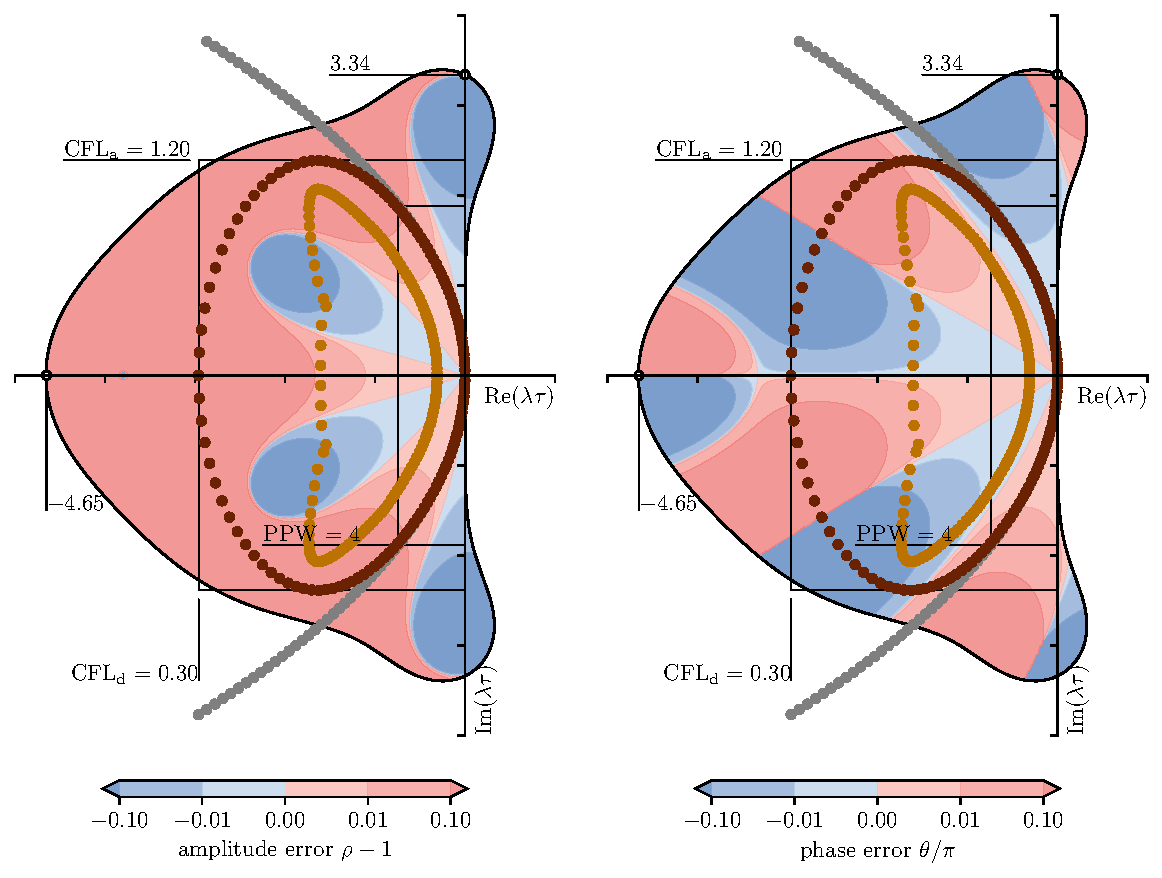
\includegraphics[clip,height=0.7\textwidth]{figs/rkm4}
  \caption{Fourth-order explicit Runge-Kutta scheme. Colored area indicates the stability region. The five zeros of the polynomial $r=r(\lambda\tau)$ are enclosed by the blue closed regions in the left panel. Markers indicate the eigenvalues for the advection-diffusion equation and $n=128$: gray, periodic case with spectral FDMs; dark brown, periodic case with compact FDMs; light brown, Dirichlet case with compact FDMs.}
  \label{fig:rkm}
\end{figure}

For the fourth-order five-step Runge-Kutta method that we use in the code, one finds (see figure~\ref{fig:rkm})
\begin{equation}
  r=1+\sum_1^4\frac{1}{k!}(\lambda \tau)^k+\frac{1}{200}(\lambda \tau)^5 \;.
\end{equation}
The equation above shows the forth-order accuracy, since the first term that deviates from the Taylor series of the exponential function is proportional to $(\lambda\tau)^5$. The crossing points of the boundary of the stability region with the real and imaginary axis are $(\lambda \tau)_{r}\simeq-4.65$ and $(\lambda \tau)_{i}\simeq\pm 3.34$. These numbers determine the maximum CFL numbers associated with the advection-diffusion equation, which is the basis for many non-reacting flows (a source term might add an additional stability constraint for). Assuming periodic boundary conditions for simplicity, we can diagonalize the original system to the set of equations
\begin{equation}
  \frac{d\hat{s}_j}{dt}=(ic\lambda_{1,j}/h -\nu\lambda_{2,j}/h^2)\hat{s}_j \;,\qquad j=0,\ldots,n-1\;,
  \label{equ:eigenvalues}
\end{equation}
according to the eigenvalue analysis discussed in section~\ref{sec:fdm}. In the expression above, $c$ is a constant representing an advection velocity and $\nu$ is the viscosity.  The expression within parenthesis is the eigenvalue $\lambda_j$ and it needs to belong to the stability region shown for the algorithm to be stable. This condition implies
\begin{equation}
  \frac{\nu\tau}{h^2}<\frac{|(\lambda \tau)_{r}|}{\max_j\{\lambda_{2,j}\}}\;,\qquad
  \frac{c\tau}{h}<\frac{|(\lambda \tau)_{i}|}{\max_j\{\lambda_{1,j}\}} \;.
\end{equation}
The left-hand sides in the expressions above are the $\textrm{CFL}$ numbers $\textrm{CFL}_\mathrm{d}$ and $\textrm{CFL}_\mathrm{a}$ for the diffusion and the advection operators, respectively. The right-hand sides provide the upper bounds $\textrm{CFL}_\mathrm{d,max}=4.65/6.86=0.68$ ($4.65/\pi^2=0.47$ if we use \cite{Lamballais:2011}) and $\textrm{CFL}_\mathrm{a,max}=3.34/1.99=1.68$ having used for $\max_j\{\lambda_{2,j}\}$ and $\max_j\{\lambda_{1,j}\}$ the values shown in figure~\ref{fig:fdm}.

Besides stability, we also want a small error. Figure~\ref{fig:rkm} shows the amplitude and phase errors as defined in (\ref{equ:rkmerror}). That figure explains the reason to use CFL numbers that are smaller than the maximum for stability. The value $\mathrm{CFL}_\mathrm{a}=0.7\,\mathrm{CFL}_\mathrm{a,max}\simeq 1.2$ is used in the code by default. In the real axis, the code uses by default $1/4$ of the limit in the imaginary axis, that is, $\textrm{CFL}_\mathrm{d}=0.3$. Wavenumbers corresponding to more than 4 PPW fall approximately within 10\% error.

For the third-order Runge-Kutta method that we use in the code, one finds (see figure~\ref{fig:rkm3})
\begin{equation}
  r=1+\sum_1^3\frac{1}{k!}(\lambda \tau)^k \;.
\end{equation}
The maximum $\mathrm{CFL}$ numbers to guarantee stability for the advection and diffusion operators are $\mathrm{CFL}_\mathrm{a,max} = 1.73/1.989=0.871$ and $\mathrm{CFL}_\mathrm{d,max} = 2.57/6.857=0.375$ ($2.57/\pi^2=0.26$ if we use \cite{Lamballais:2011}), respectively. The value $\mathrm{CFL}_\mathrm{a}=0.7\,\mathrm{CFL}_\mathrm{a,max}\simeq 0.6$ is used in the code by default. In the real axis, the code uses by default $1/4$ of the limit in the imaginary axis, that is, $\textrm{CFL}_\mathrm{d}=0.15$.

\begin{figure}[!ht]
  \centering
  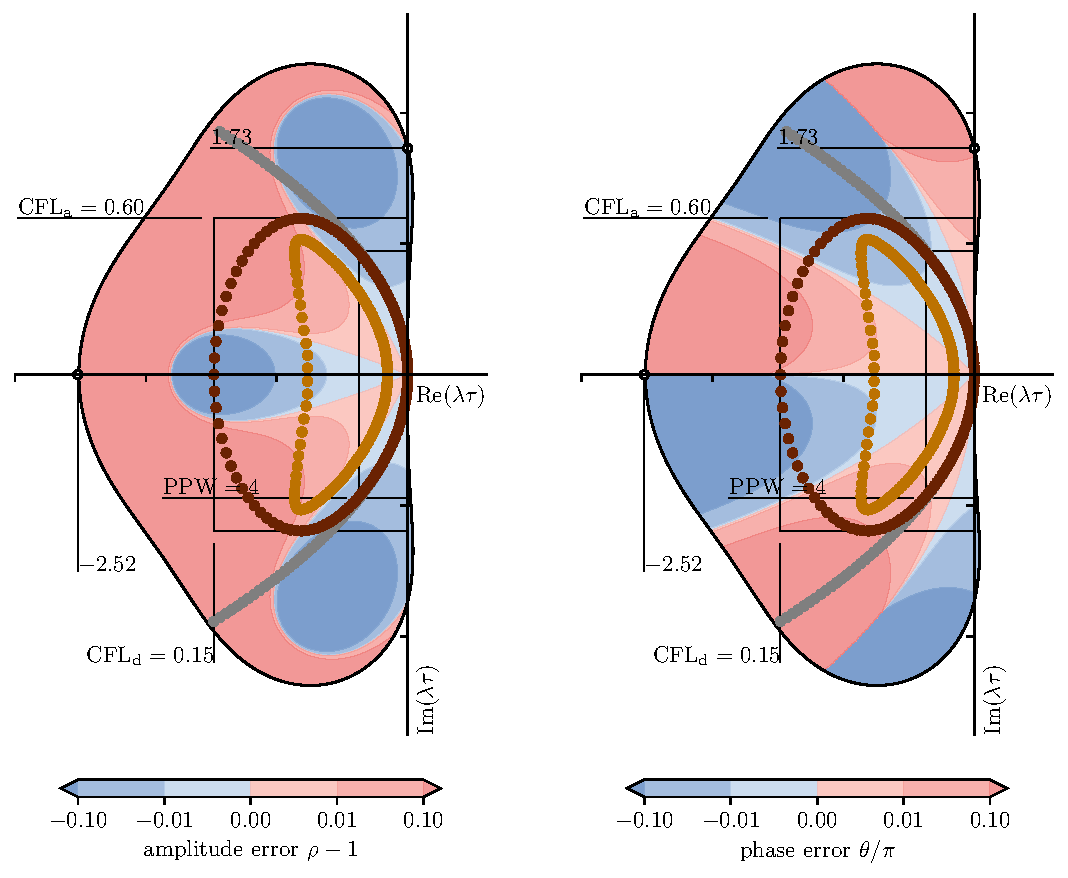
\includegraphics[clip,height=0.7\textwidth]{figs/rkm3}
  \caption{Third-order explicit Runge-Kutta scheme. Colored area indicates the stability region. The five zeros of the polynomial $r=r(\lambda\tau)$ are enclosed by the blue closed regions in the left panel. Markers indicate the eigenvalues for the advection-diffusion equation and $n=128$: gray, periodic case with spectral FDMs; dark brown, periodic case with compact FDMs; light brown, Dirichlet case with compact FDMs.}
  \label{fig:rkm3}
\end{figure}

We have considered the periodic case, which is easier because the eigenvalues can be obtained analytically and both the diffusion and advection operator have the same eigenvectors. For the non-periodic case, we generally need to calculate the eigenvalues numerically.  For instance, let us consider the advection equation inside the domain $[x_1,x_n]$ with a positive advection velocity $u$ and (therefore) the boundary condition imposed at the left boundary $x_1$, that is
\begin{equation}
  \left.\begin{array}{ll}
  d\mathbf{s}/dt|_j = -c\; \delta_x \mathbf{s}|_j & j=2,\ldots,n\\
  s_1=\alpha
  \end{array}\right\} \;,\qquad c\ge 0  \;.
  \label{equ:problem2}
\end{equation}
We know that $\delta_x \mathbf{s} = (1/2)A_1^{-1}B_1\mathbf{s}$, but we only need a relation involving the last $n-1$ components of the vector $\mathbf{s}$, not all of them. This can be obtained by introducing the following block matrices \citep{Lomax:1998,Mellado:2012}
\begin{equation*}
  A_1=
  \left(\begin{array}{cc}a_{11}&\mathbf{a_{12}}^T \\\mathbf{a_{21}}   &A_{22}\\
  \end{array}\right) \;, \qquad
  B_1=
  \left(\begin{array}{cc}b_{11}&\mathbf{b_{12}}^T \\\mathbf{b_{21}}   &B_{22}\\
  \end{array}\right) \;.
\end{equation*}
Then, eliminating $s'_1$ in the original system, yields
\begin{equation}
  hA^R_{22}
  \left(\begin{array}{c}s'_2\\\vdots\\s'_n\end{array}\right) =
  B^R_{22}\left(\begin{array}{c}s_2\\\vdots\\s_n\end{array}\right)+
  s_1\mathbf{b^R_{21}} \;,
\end{equation}
where the $(n-1)\times (n-1)$ matrices $\{A^R_{22}\,,B^R_{22}\}$ and the column vector $\mathbf{b^R_{21}}\in\mathbb{R}^{n-1}$ are
\begin{equation}
  A^R_{22}=A_{22}-\frac{1}{a_{11}}\mathbf{a_{21}}\mathbf{a_{12}}^T \;,\qquad
  B^R_{22}=B_{22}-\frac{1}{a_{11}}\mathbf{a_{21}}\mathbf{b_{12}}^T \;,\qquad
  \mathbf{b^R_{21}}=\mathbf{b_{21}}-\frac{b_{11}}{a_{11}}\mathbf{a_{21}} \;.
\end{equation}
Note that $A^R_{22}$ and $B^R_{22}$ have the same bandwidths as $A$ and $B$, respectively. The element $s'_1$ can be calculated by
\begin{equation}
  s'_1=\frac{1}{ha_{11}}
  \left(\begin{array}{cc}b_{11}\!&\!\mathbf{b_{12}}^T\end{array}\right)
  \mathbf{s} - \frac{1}{a_{11}}
  \mathbf{a_{12}}^T \left(\begin{array}{c}s'_2\\\vdots\\s'_n\end{array}\right)\;.
\end{equation}

% \begin{SCfigure}
% \includegraphics[clip,width=0.45\textwidth]{figs/AdvectionSpectra}
% \caption{Spectra of the matrix $-\{(A^R_{22})^{-1}B^R_{22}\}$ describing the
%   advection operator in problem (\ref{equ:problem2}) for two different problem
%   sizes: black, $n=32$; ref, $n=1024$. As the number of grid points is
%   increased, the role of the boundary conditions decrease and the spectra tends
%   towards that corresponding to periodic boundary conditions, which is purely
%   imaginary (see figure~\ref{fig:fdm}). Note, however, that deviation from the
%   imaginary axis of the eigenvalues is relatively small even for the small size
%   $n=32$, in the context of the dissipation- and dispersion-error regions shown
%   in figure~\ref{fig:rkm}.}\label{fig:advection}
% \end{SCfigure}

Then, the original equation can be written as
\begin{equation}
  \frac{d}{dt}
  \left(\begin{array}{c}s_2\\\vdots\\s_n\end{array}\right) =
  -(c/h)(A^R_{22})^{-1}B^R_{22}\left(\begin{array}{c}s_2\\\vdots\\s_n\end{array}\right)+
  \alpha\mathbf{b^R_{21}} \;,
\end{equation}
so that the set of complex numbers $-(c\tau/h) \textrm{eig} \{(A^R_{22})^{-1}B^R_{22}\}$ have to fall inside the stability region. \citep{Carpenter:1993}.

The same can be done for the diffusion operator. In this case, we impose 2 boundary conditions. If one of the boundary conditions is imposed at $x=x_n$, then we need to eliminate $s_n$ as we have eliminated before $s_1$ when the boundary condition is imposed at $x=x_1$. We obtain now reduced matrices of size $(n-2)\times(n-2)$. For the compact schemes used in the code, this analysis shows that the CFL conditions derived from the spectral FDM approximations are also applicable to the biased schemes used in non-periodic directions, as observed in figure~\ref{fig:rkm}.

%This set of eigenvalues is shown in figure~\ref{fig:advection} for the scheme (35653) used in the code by default, normalized by the prefactor $u\tau/h$. We see that the spectra is dominated by a form relatively close to that of the periodic boundary conditions, which was purely imaginary, and the CFL condition is therefore the same. It happens that some other biased FD formulae at the boundary points can mode part of the spectra into the positive real part of the complex plane, which would lead to unstable algorithms \citep{Carpenter:1993}.

In case of a nonuniform grid, we need to consider the diagonal matrices $D_1$ and $D_2$ in (\ref{equ:nonuniform1}) and (\ref{equ:nonuniform2}). The effect of a varying grid spacing can be studied with the script \texttt{figure.py}. When we use the minimum of grid spacing in the CFL definitions, part of the eigenvalues approach the origin from the stable side.

For the multidimensional case, we need to consider the sum of all possible combinations of eigenvalues in each direction \citep{Lomax:1998}.

\subsection{Implicit schemes}

To be developed. See \cite{Spalart:1991}.

The dissipation and dispersion error maps corresponding to the third-order implicit Runge-Kutta scheme are shown in figure~\ref{fig:rkm3implicit}. The algorithm is unconditionally stable but we need to control accuracy of the diffusion operator for which it is used. The reference value $\textrm{CFL}_d=1.7$ as it gets most of the eigenvalues within the 1\%-error region.

\begin{figure}
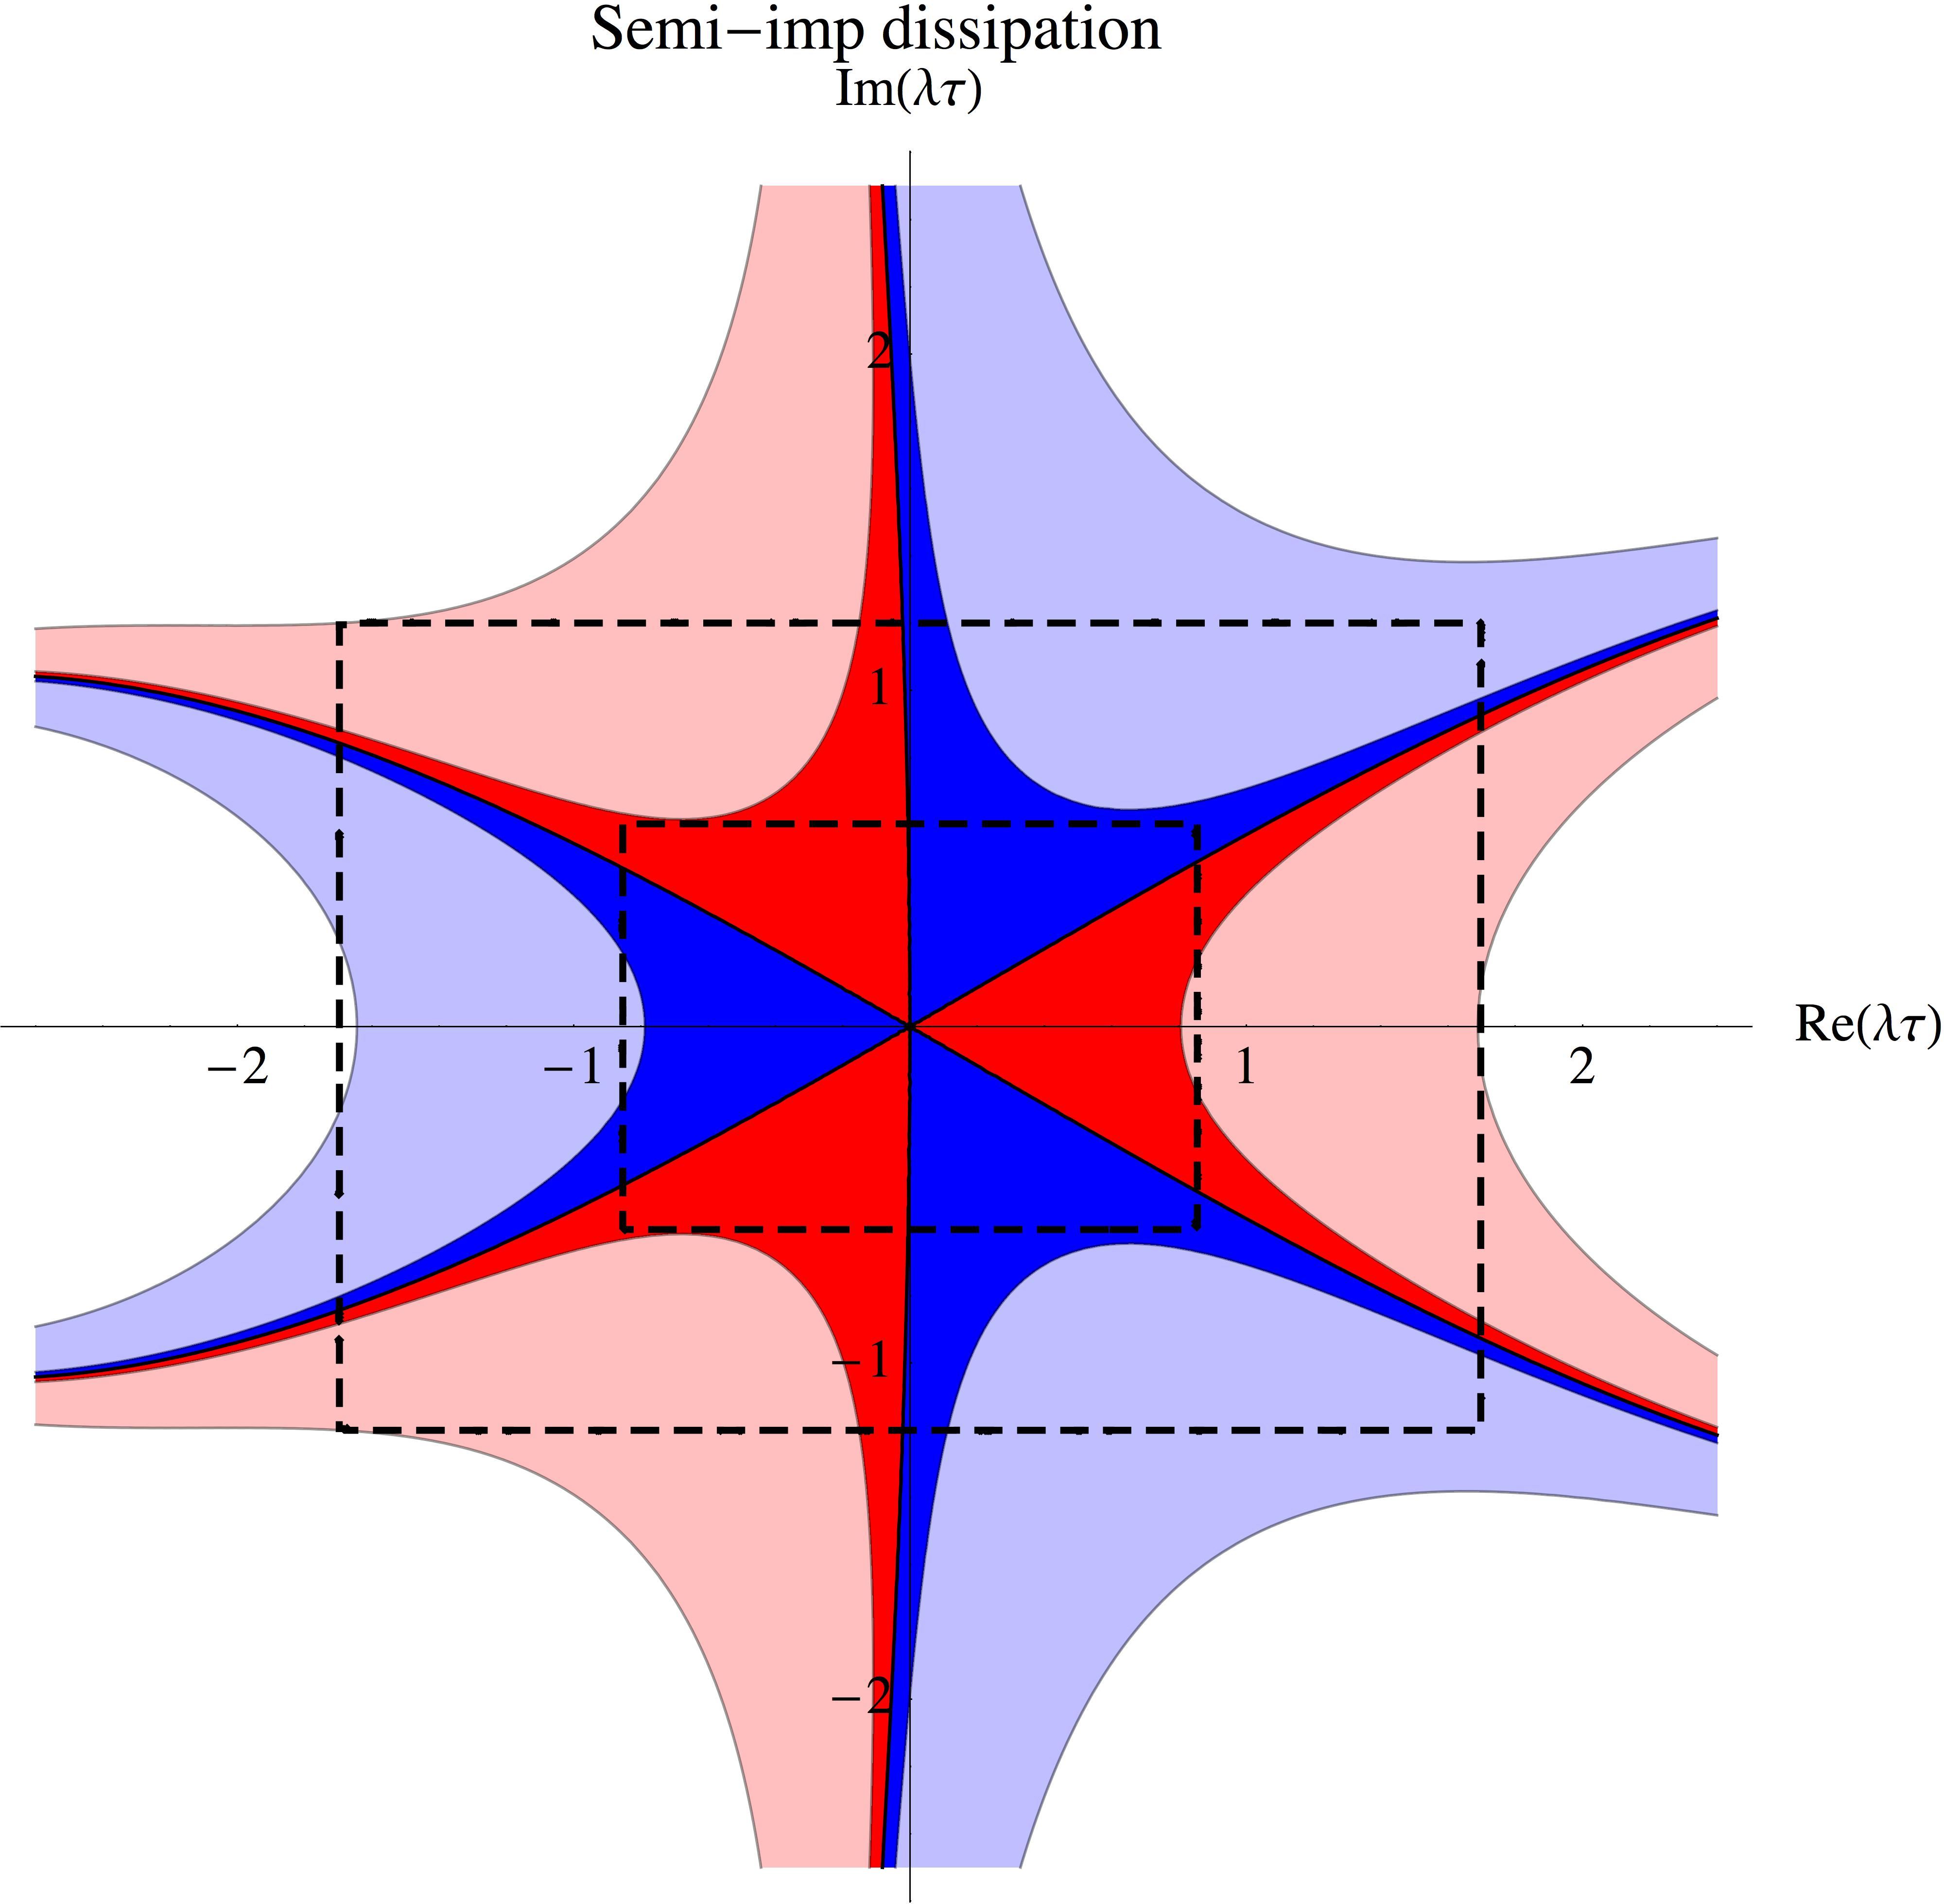
\includegraphics[clip,width=0.49\textwidth]{figs/RK3_imp_diss.jpg}\hfill
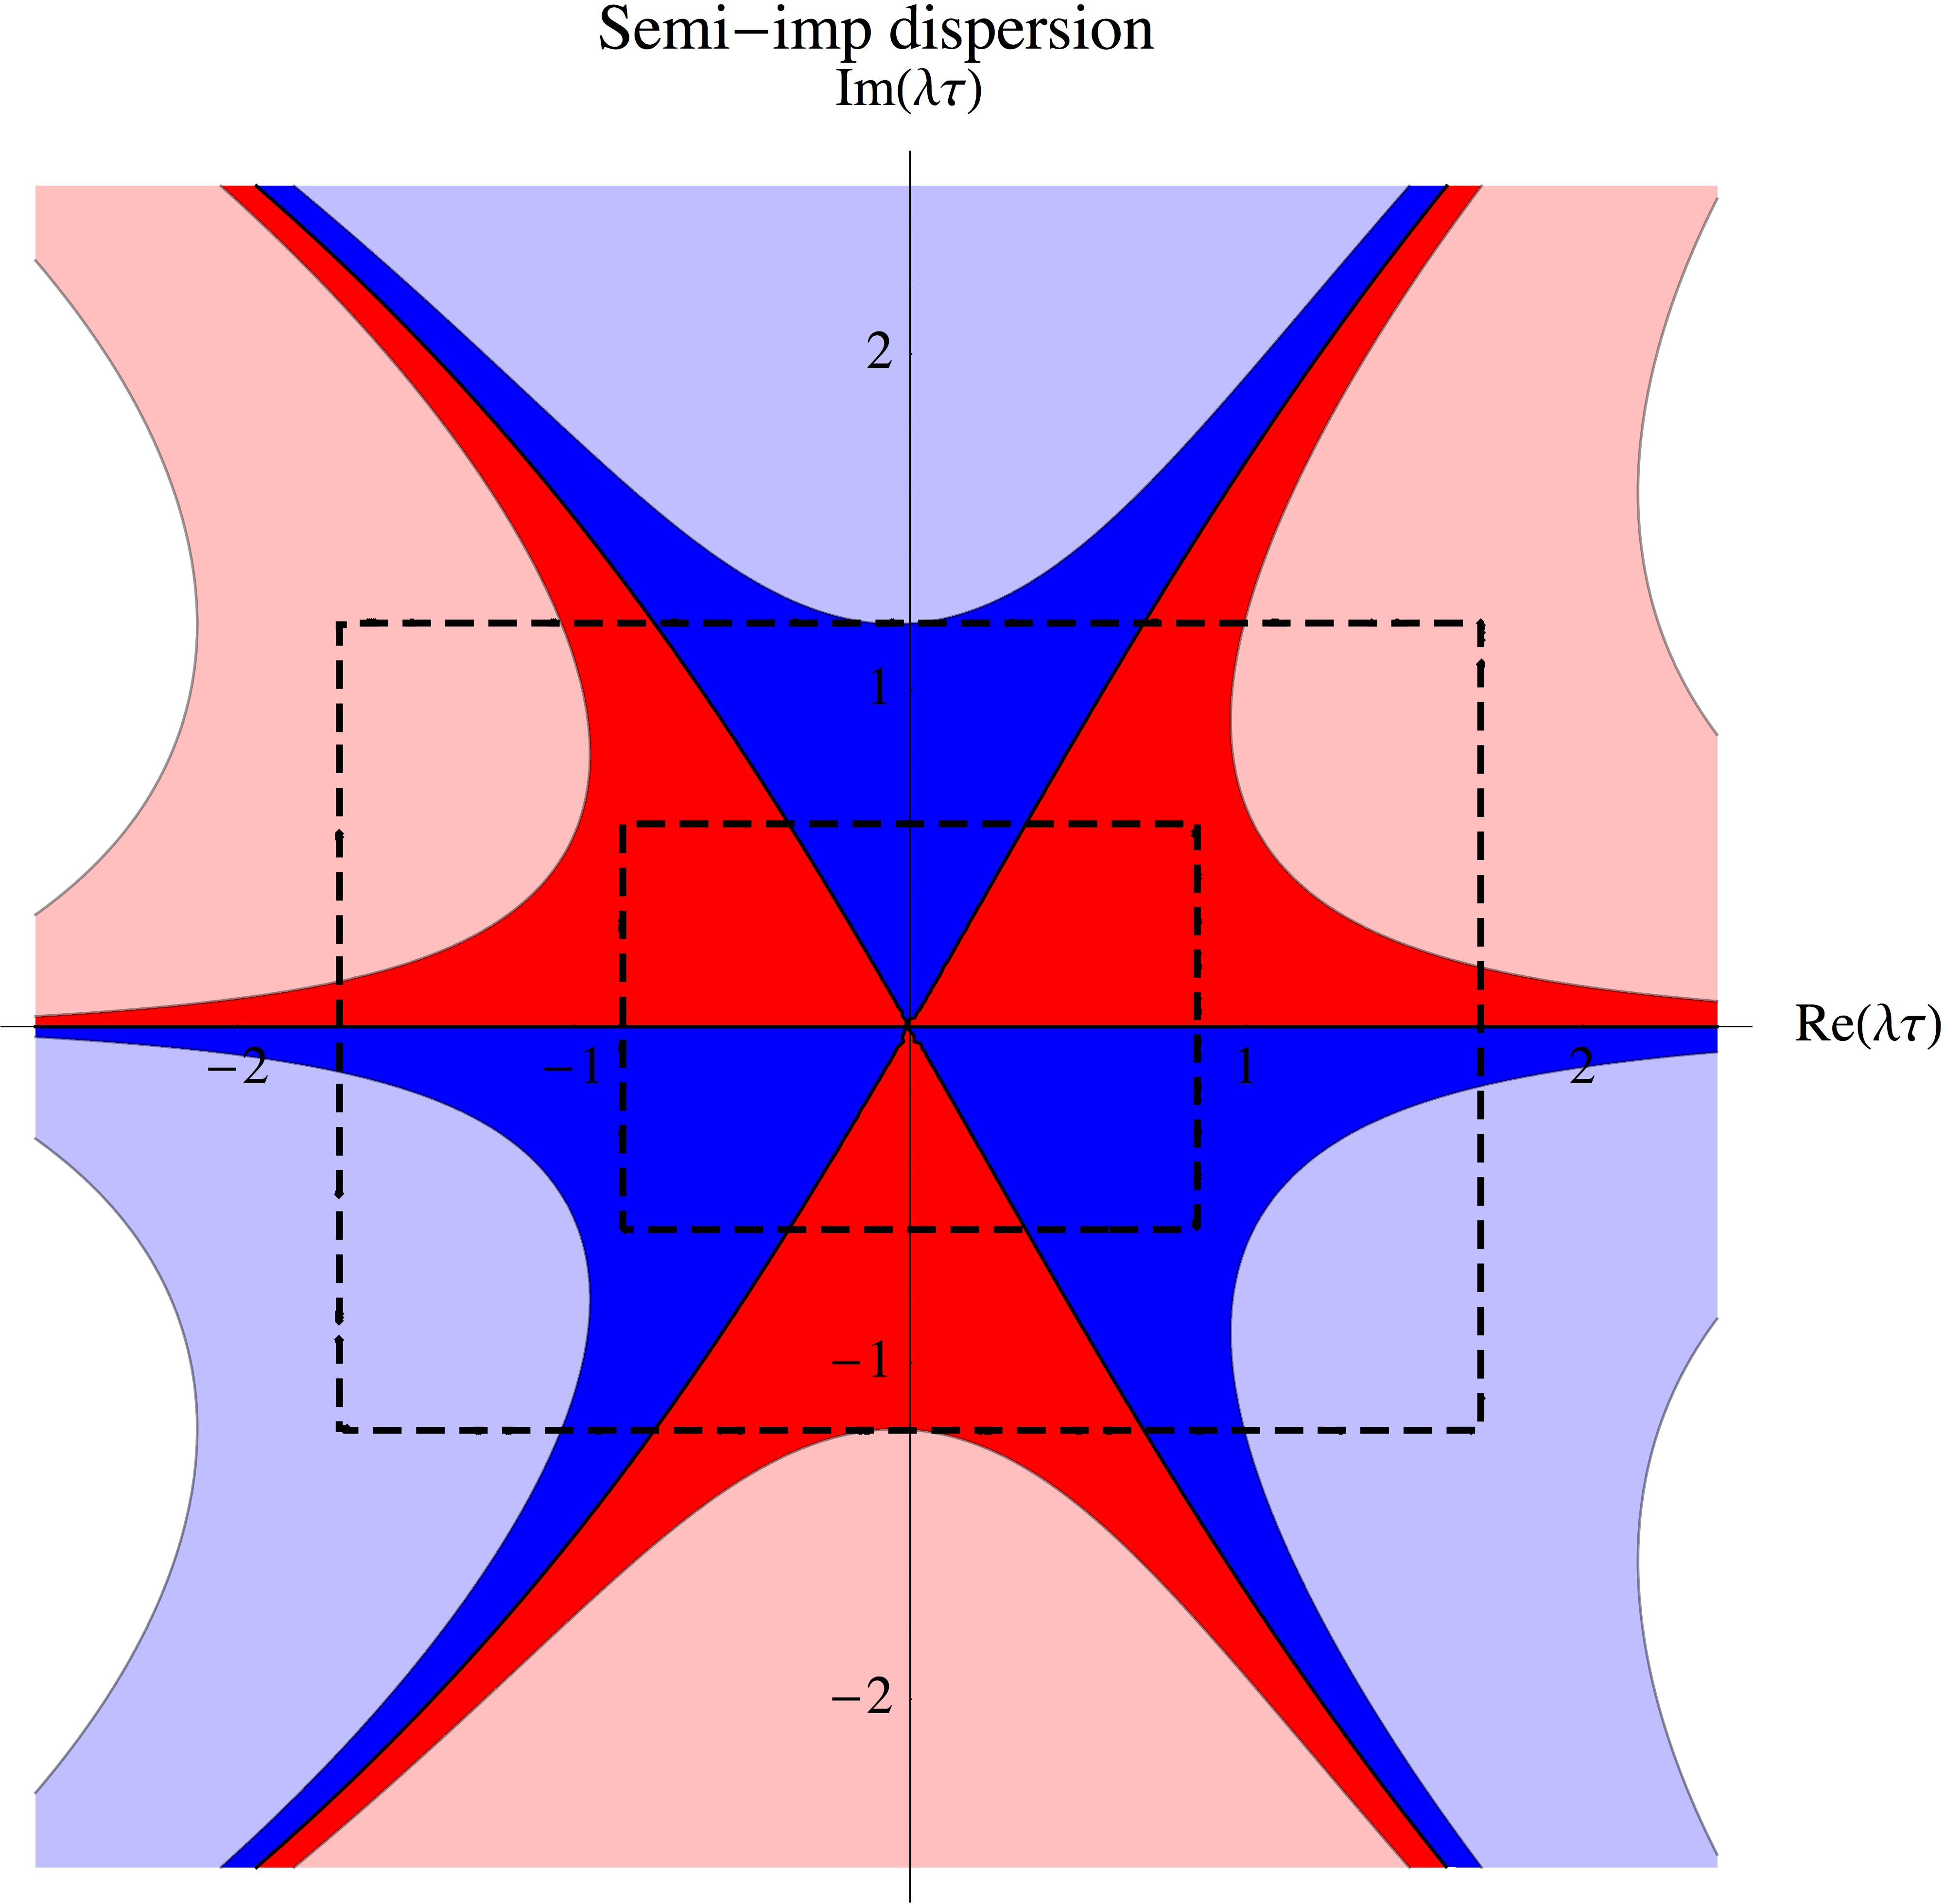
\includegraphics[clip,width=0.49\textwidth]{figs/RK3_imp_disp.jpg}
\caption{Dissipation error (left) associated with the third-order implicit
  Runge-Kutta scheme: dark blue, $0.99<\rho<1$; light blue, $0.90<\rho<0.99$;
  dark red, $1<\rho<1.01$; light red, $1.01<\rho<1.10$. Dispersion error (right)
  associated with the Runge-Kutta scheme: dark blue, $-0.01<\theta/\pi<0$; light
  blue, $-0.10<\theta/\pi<-0.01$; dark red, $0<\theta/\pi<0.01$; light red,
  $0.01<\theta/\pi<0.10$.}\label{fig:rkm3implicit}
\end{figure}
